\section{Results}
\label{sec:results}

\subsection{Thesis protocol: random split}
Table~\ref{tab:metrics} and Fig.~\ref{fig:parity} show the test-set performance of the thesis models on the random 80/20 split. The three non-linear models reach $R^2 > 0.96$, with Random Forest best on every metric. Ridge regression fails at high solubility, where the dependence on pressure is strongly non-linear. These numbers use the thesis descriptors and a split in which nearly every test IL is also in the training set, and 29\% of the test points have an identical copy in the training set (Section~\ref{sec:issues}); Section~\ref{sec:grouped} shows that they overstate the accuracy for new ILs.

\begin{table}[t]
\caption{Thesis protocol: test-set performance of the four models on the thesis set with the thesis descriptors (random 80/20 split, 2,252 test points). MAE and RMSE are in mole fraction. Training times are for one fit on a laptop CPU.}
\label{tab:metrics}
\centering
\begin{tabular}{lcccc}
\toprule
\textbf{Model} & $R^2$ & \textbf{MAE} & \textbf{RMSE} & \textbf{Training time (s)} \\
\midrule
Random Forest & 0.9853 & 0.0167 & 0.0275 & 1.0 \\
Gradient Boosting & 0.9729 & 0.0257 & 0.0374 & 1.1 \\
Neural network & 0.9656 & 0.0346 & 0.0422 & 19.7 \\
Ridge regression & 0.5906 & 0.1164 & 0.1455 & 0.1 \\
\bottomrule
\end{tabular}
\end{table}

\begin{figure}[t]
\centering
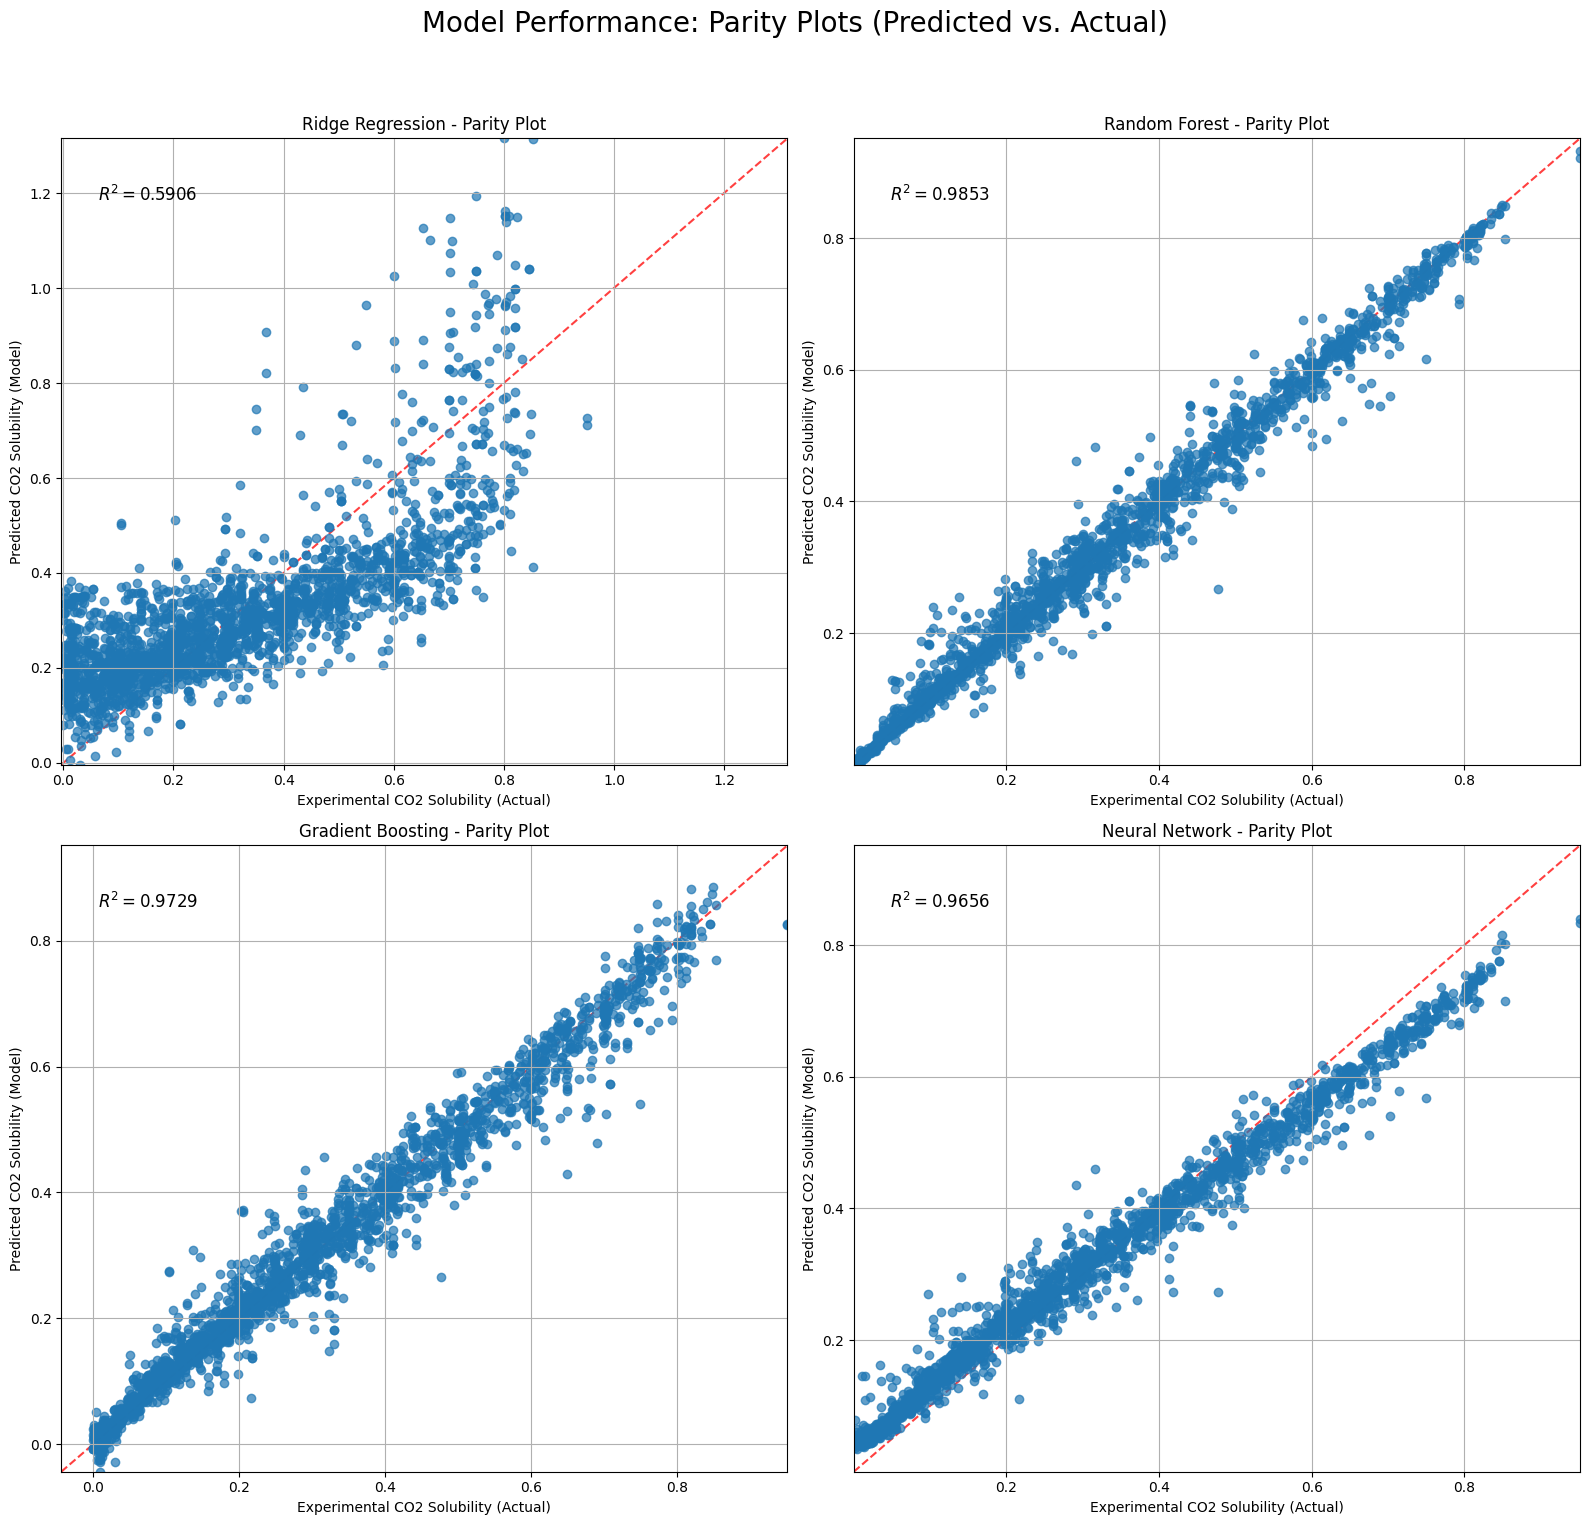
\includegraphics[width=0.8\textwidth]{figures/fig_parity_thesis.png}
\caption{Thesis protocol: predicted against experimental \co{} solubility on the random test set for the four models. The dashed line marks perfect agreement.}
\label{fig:parity}
\end{figure}

\subsection{Grouped validation and descriptor comparison}
\label{sec:grouped}
Table~\ref{tab:grouped} and Fig.~\ref{fig:grouped} give the results of the main protocol on the curated dataset. Four observations stand out.

\begin{table}[t]
\caption{Main protocol: 5-fold cross-validation on the curated dataset (12,026 points, 110 ILs). $R^2$ is the mean $\pm$ standard deviation over the folds; MAE (mole fraction) is the fold mean for leave-anion-out. RF: Random Forest; GB: histogram gradient boosting. Counts: elemental atom counts.}
\label{tab:grouped}
\centering
\small
\setlength{\tabcolsep}{5pt}
\begin{tabular}{llcccc}
\toprule
 & & \multicolumn{3}{c}{\textbf{$R^2$}} & \textbf{MAE} \\
\cmidrule(lr){3-5} \cmidrule(lr){6-6}
 & \textbf{Features ($T$, $P$ +)} & \textbf{Point-wise} & \textbf{Leave-IL-out} & \textbf{Leave-anion-out} & \textbf{Leave-anion-out} \\
\midrule
RF & --- & 0.848 & $0.833 \pm 0.033$ & $0.773 \pm 0.062$ & 0.075 \\
 & counts & 0.982 & $0.953 \pm 0.014$ & $0.873 \pm 0.030$ & 0.054 \\
 & thesis DFT & 0.981 & $0.951 \pm 0.011$ & $0.841 \pm 0.109$ & 0.055 \\
 & corrected DFT & 0.983 & $0.953 \pm 0.018$ & $\mathbf{0.896 \pm 0.016}$ & 0.052 \\
 & thesis DFT + counts & 0.983 & $0.955 \pm 0.013$ & $0.843 \pm 0.111$ & 0.057 \\
 & corrected DFT + counts & 0.983 & $0.955 \pm 0.015$ & $0.890 \pm 0.019$ & 0.053 \\
\midrule
GB & --- & 0.871 & $0.854 \pm 0.028$ & $0.801 \pm 0.058$ & 0.071 \\
 & counts & 0.990 & $0.968 \pm 0.008$ & $0.906 \pm 0.026$ & 0.047 \\
 & thesis DFT & 0.990 & $0.959 \pm 0.018$ & $0.887 \pm 0.073$ & 0.046 \\
 & corrected DFT & 0.990 & $0.960 \pm 0.017$ & $\mathbf{0.925 \pm 0.018}$ & 0.043 \\
 & thesis DFT + counts & 0.990 & $0.968 \pm 0.009$ & $0.884 \pm 0.070$ & 0.050 \\
 & corrected DFT + counts & 0.990 & $0.964 \pm 0.012$ & $0.922 \pm 0.020$ & 0.043 \\
\bottomrule
\end{tabular}
\end{table}

\begin{figure}[t]
\centering
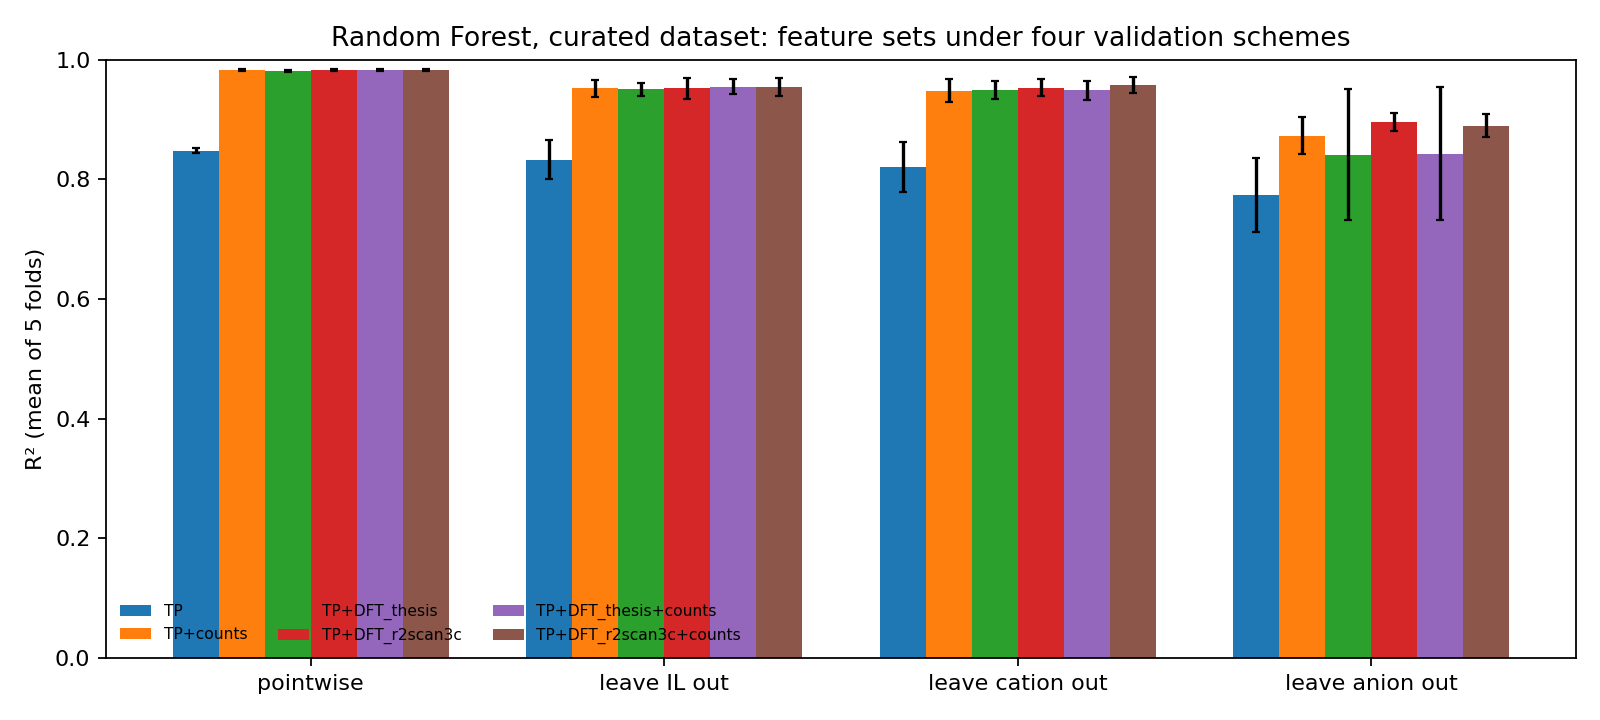
\includegraphics[width=0.95\textwidth]{figures/fig_grouped_validation.png}
\caption{Random Forest $R^2$ (mean of five folds, error bars one standard deviation) for the six feature sets under the four validation schemes on the curated dataset.}
\label{fig:grouped}
\end{figure}

\textit{The random split does not discriminate.} Every feature set that identifies the ions scores $R^2 = 0.98$--$0.99$ point-wise, whether its DFT descriptors are correct or not. Holding out whole ILs lowers $R^2$ to 0.95--0.97, and holding out whole anions to 0.84--0.93.

\textit{Ion information is essential.} Temperature and pressure alone give $R^2 = 0.77$--0.80 for unseen anions. Any description of the ions adds 0.07--0.12.

\textit{The corrected descriptors are clearly better than the thesis descriptors.} For unseen anions, $R^2$ rises from 0.84 to 0.90 (Random Forest) and from 0.89 to 0.93 (gradient boosting), and the fold-to-fold standard deviation falls from 0.07--0.11 to about 0.02. Adding the thesis descriptors to the atom counts makes both models worse for unseen anions (0.84 against 0.87 for Random Forest, 0.88 against 0.91 for gradient boosting), so the thesis descriptors behaved partly as noise.

\textit{The corrected isolated-ion descriptors are slightly better than atom counts.} For unseen anions, ten corrected DFT descriptors give $R^2 = 0.90$ against 0.87 for fifteen atom counts with Random Forest, and 0.93 against 0.91 with gradient boosting. Because all feature sets share the same folds, the comparison can be made fold by fold: the DFT descriptors are better in four of the five folds for both models, by 0.02 on average, and marginally worse (by less than 0.01) in the fifth. Combining them with the atom counts adds nothing. The gain is small, and much of what the descriptors convey is still the size and identity of each ion; their further advantages are physical meaning and the ability to describe ions with elements or bonding not present in the training set. On the first ILThermo build, before the corrections of Section~\ref{sec:curated}, the two feature sets were indistinguishable.

\subsection{Anions that are hard to predict}
For gradient boosting with the corrected descriptors, the largest leave-anion-out errors are for [NfO]$^-$ (mean absolute error 0.10 in mole fraction, 48 points), [MeSO$_3$]$^-$ (0.08, 261 points), [TCB]$^-$ (0.08, 130 points), [MeSO$_4$]$^-$ (0.07, 380 points), [NO$_3$]$^-$ (0.06, 243 points) and [TFA]$^-$ (0.06, 138 points). Five of the six are oxygen-donor anions (sulfonates, a sulfate, nitrate and a carboxylate), whose interaction with \co{} may differ from that of the fluorinated anions that dominate the data. Each occurs with only two to seven cations, but so do several anions that are predicted well, so the small number of cations alone does not explain the errors. The largest improvement from the corrected descriptors is for [SCN]$^-$, whose error falls from 0.16 with the thesis descriptors to 0.04.

\subsection{Feature importance in the thesis models}
Fig.~\ref{fig:importance} shows permutation importances of the thesis Random Forest and Gradient Boosting models on the random test set, excluding atom counts. Pressure dominates, followed by temperature and the anion total energy. Because these models use the thesis descriptors and a random split, the ranking of the DFT descriptors should not be interpreted physically; the total energy in particular scales with the size and composition of an ion and acts largely as an identifier. Importances for the corrected descriptors under grouped validation will be reported with the next descriptor set (Section~\ref{sec:summary}).

\begin{figure}[t]
\centering
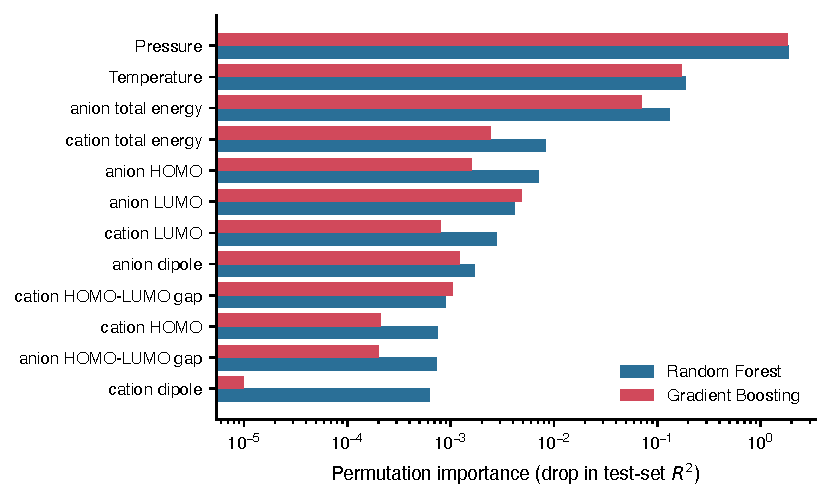
\includegraphics[width=0.75\textwidth]{figures/fig_importance.pdf}
\caption{Thesis models: permutation importance of temperature, pressure and the ten thesis DFT descriptors for Random Forest and Gradient Boosting (random test set, 10 repeats, logarithmic scale). Atom counts are omitted.}
\label{fig:importance}
\end{figure}
